\fancyhf{}
\pagestyle{fancy}
%Encabezado
\lhead[]{\leftmark}
\chead[]{}
\rhead[]{\thepage}
\renewcommand{\headrulewidth}{1pt}

\section{Introducción}

En el capítulo anterior, se explicó la importancia de analizar ids ubicados en los códigos. Los ids de un programa normalmente están compuestos por más de una palabra en forma de abreviatura, por ejemplo: \textsf{inp\_fl\_sys}. Detrás de estas abreviaturas, los ids ocultan información es propia del Dominio del Problema \cite{BCPT99,LFBEX07,EZH08,EHPV09}. Desafortunadamente, las personas ajenas al código, no comprenden a simple vista la información que los ids poseen en sus abreviaturas e invierten tiempo en entenderlas. Es por esto, que las herramientas automáticas de análisis de ids son bienvenidas en el ámbito de la Comprensión de Programas (CP). Con estas herramientas se logra disminuir los tiempos de comprensión de ids y revelar la información que estos contienen en sus abreviaturas.

Dada la importancia que tienen las herramientas de análisis de ids, se tomó la iniciativa de desarrollar una llamada Identifier Analyzer (IDA). Esta herramienta le permite al usuario ingresar un archivo JAVA, luego IDA analiza los ids que están en el archivo.
%, y finalmente produce como resultado una tabla del análisis realizado, esta tabla contiene los ids encontrados en el programa pero expandidos. 
La forma en que IDA analiza los ids, se efectuá en tres pasos: I) Extraer los ids del código de estudio. II) Aplicar una técnica de división, en donde se descompone al id en las distintas abreviaturas que lo componen. Por ejemplo: \textsf{inp\_fl\_sys} $\rightarrow$ \textsf{inp fl sys}. \linebreak III) Por último, emplear una técnica de expansión de abreviaturas que las expande a palabras completas. Por ejemplo: \textsf{inp fl sys} $\rightarrow$ \textsf{input file system}. Una vez realizado los tres pasos, los resultados de las expansiones de ids se exhiben en una tabla.
El objetivo de IDA es lograr que el usuario comprenda más rápidamente el propósito de los ids en los archivos JAVA, y de esta manera mejorar la comprensión del código analizado.

%Para que IDA pueda realizar su tarea, contiene implementados 2 algoritmos de división de ids (Greedy y Samurai) y 1 algoritmo de expansión de abreviaturas (Expansión Básica), los mismos fueron explicados en el capítulo precedente. 

El correspondiente capítulo, está destinado a explicar los distintos módulos que IDA posee, y que proceso de ejecución debe realizar el usuario para analizar los ids. Al final de este capítulo, se describen algunos casos de estudio que demuestran la importancia de haber construido IDA. Todas estas explicaciones, están acompañadas con capturas de pantalla y tablas que facilitarán al lector entender el funcionamiento de la herramienta IDA. 
Para comenzar con la descripción de IDA, en la siguiente sección se explica la arquitectura y cuales son sus componentes principales.

%La herramienta IDA le permite al usuario ingresar archivos con código JAVA. Luego la herramienta ejecuta técnicas/algoritmos que analizan los ids situados en el código del archivo.

%La herramienta IDA le permite al usuario revelar la información estática oculta que hay detrás de los ids. Esto se logra mediante la ejecución de técnicas/algoritmos que fueron descriptos en el capítulo anterior.
%
%La iniciativa del desarrollo de la herramienta IDA surgió, porque en la actualidad no existe otra herramienta en el ámbito de la CP con similares características.

%El objetivo de aplicar estas técnicas consiste en convertir los ids que están abreviados a palabras completas más entendibles para el lector ajeno al código.

%Una vez realizada esta conversión, IDA le permite al usuario reemplazar a elección los ids con los nuevos nombres, creando así un nuevo archivo con código más legible y sin alterar la funcionalidad original del código. 

\begin{figure}[t] %[h] para here [b] para bottom [t] para top
\centerline{%queda centrada mejor la imagen
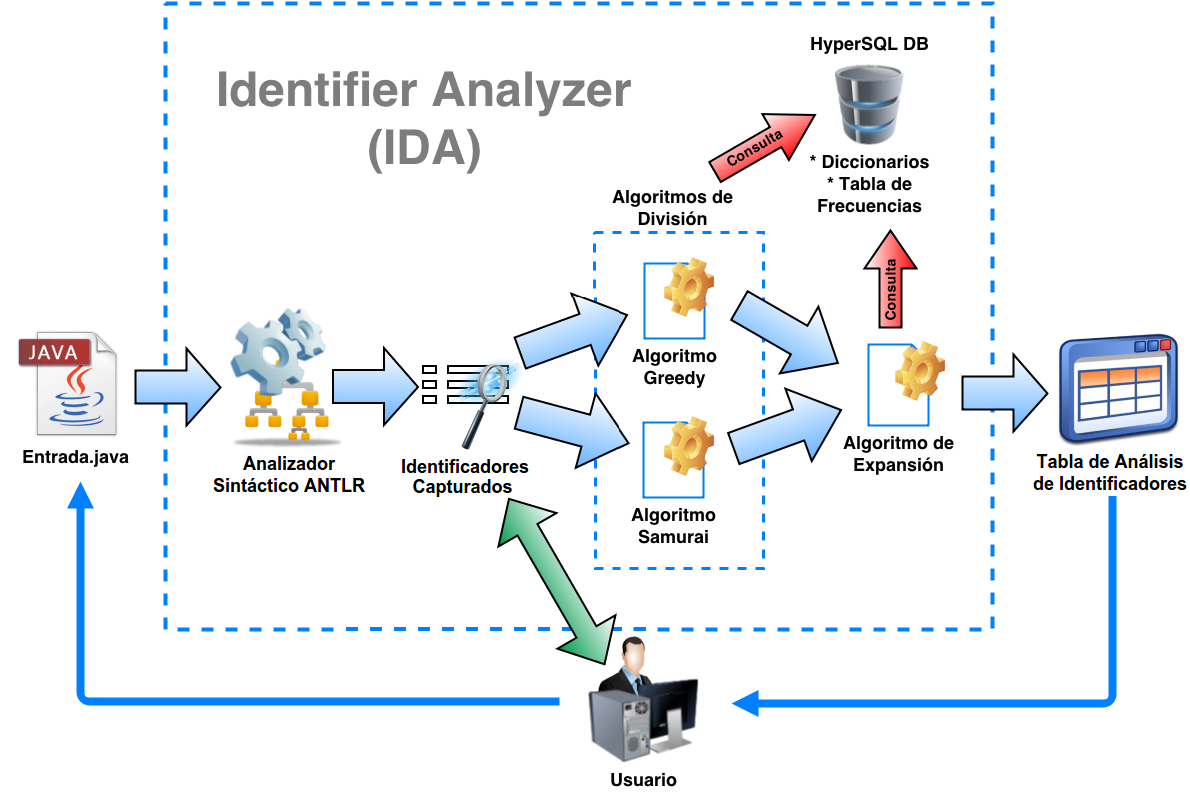
\includegraphics[scale= 0.35]{./cap4/ida_arq.png}
}
\caption{Arquitectura de IDA.}
\label{arq1}
\end{figure}


\section{Arquitectura}

%La herramienta IDA se implementó empleando lenguaje JAVA y se programó usando el entorno de desarrollo NetBeans\footnote[1]{https://www.netbeans.org}. 

En la figura \ref{arq1} se puede apreciar la arquitectura de IDA. Esta arquitectura describe tres partes principales, la primera consiste en la \textit{extracción de datos}, la segunda trata sobre la \textit{división de ids} y la tercera sobre \textit{expansión de ids}. A continuación se detallan cada una de ellas.\\

\textbf{Módulo de Extracción de Datos:} Este módulo recibe como entrada un archivo JAVA que ingresa el usuario (ver Figura \ref{arq1} Entrada.java), luego este archivo se procesa por un Analizador Sintáctico (AS) (\mbox{ver Figura \ref{arq1}} Analizado Sintáctico ANTLR). El AS, extrae y almacena en estructuras internas la información estática perteneciente al código del archivo ingresado. Esta información, está relacionada con ids, literales y comentarios (ver próxima sección para más detalles). El usuario a través de la interfaz de IDA, puede visualizar esta información capturada del código por medio de tablas claramente definidas (ver figura \ref{arq1} - Flecha Verde).

\textbf{Módulo de División de Ids:} Una vez completada la extracción de información, el proceso continua en el módulo de división de ids. Aquí se encuentran implementados dos algoritmos de división; uno es el Algoritmo Greedy y el otro es el Algoritmo Samurai ambos explicados en la sección \ref{sec:algGre} y \ref{sec:algSamu} del capítulo anterior. Estos algoritmos reciben como entrada la información capturada en el módulo de extracción de datos (ids, comentarios, literales), y luego estos algoritmos dividen los ids del archivo JAVA (ver figura \ref{arq1} - Algoritmos de División). Los resultados de las divisiones se almacenan en estructuras internas que serán utilizadas por el módulo de expansión. Cabe recordar que estos algoritmos de división necesitan datos externos para funcionar, uno es el diccionario de palabras (en caso de Greedy) y el otro es lista de frecuencias globales de aparición de palabras (en caso de Samurai). Estos datos externos se encuentran almacenados en una base de datos embebida (ver Figura \ref{arq1} HyperSQL DB).

\textbf{Módulo de Expansión de Ids:} La tercera y última parte, tiene implementado el Algoritmo de Expansión Básico de abreviaturas que fue explicado en la sección \ref{sec:algExpBas} del capítulo anterior. 

Este algoritmo, toma como entrada los ids separados en el módulo de división de ids (tanto de Greedy como de Samurai), luego el Algoritmo de Expansión expande las abreviaturas resultantes producto de la división de ids (ver Figura \ref{arq1} - Algoritmo de Expansión). Los resultados de las expansiones se retornan en dos grupos: las expansiones provistas por el Algoritmo de división Greedy y las provistas por el Algoritmo de división Samurai.

%En este punto, el usuario podrá elegir que expansión es la más adecuada y reemplazar los ids originales en el archivo de entrada, generando de esta manera un nuevo archivo de salida (ver figura \ref{arq1} Salida.java). 

El \mbox{Algoritmo} de Expansión también necesita de un diccionario de palabras, por eso se realizan consultas a la base de datos embebida (ver Figura \ref{arq1} - HyperSQL DB). Finalmente, los resultados de las divisiones y las expansiones de los ids, se muestran en una tabla (ver Figura \ref{arq1} - Tabla de análisis de identificadores).

\section{Analizador Sintáctico}

Como se explicó en la sección previa, cuando el usuario ingresa un archivo JAVA, IDA examina y extrae información estática presente en el archivo ingresado. Esta información está compuesta por identificadores, comentarios y literales. La manera en que IDA extrae esta información es a través de un Analizador Sintáctico (AS).

La construcción de este AS se llevó a cabo, primero investigando herramientas encargadas de construir AS. Se dio preferencia a aquellas que emplean la teoría asociada a las gramáticas de atributos \cite{AHUL06}. De la investigación previamente descripta, se determinó que la herramienta \textit{ANTLR}\footnote[1]{ANother Tool for Language Recognition. http://www.antlr.org} era la que mejor se ajustaba a las necesidades antes planteadas. 
Esta herramienta permite agregar acciones semánticas (escritas en JAVA) para el cálculo de los atributos, en una gramática de lenguaje JAVA\footnote[2]{http://docs.oracle.com/javase/specs/jls/se7/jls7.pdf}. Estas acciones semánticas deben estar correctamente insertadas en la gramática para, por ejemplo, implementar estructuras de datos y algoritmos que capturan los ids utilizados en un programa \cite{AAJU83}. Una vez insertadas estas acciones, ANTLR lee la gramática y genera el AS adicionando acciones que fueron programadas. De esta manera, se obtiene un AS que recolecta ids mientras examina el código. A su vez a estas acciones semánticas, se le agregan otras acciones que extraen comentarios y literales strings. Estos elementos son necesarios ya que sirven para los algoritmos de análisis de ids que serán explicados en próximas secciones.

\section{Base de Datos Embebida}
\label{sec:bseEmb}

Como se describió en secciones previas, IDA posee una base de datos embebida. Esta base de datos utiliza una tecnología llamada HSQLDB\footnote[1]{Hyper SQL Data Base. http://www.hsqldb.org}. Dado que HSQLDB esta desarrollada en JAVA, al momento de incorporarla en IDA (que está programada en JAVA) no resulto una tarea difícil.
Otra ventaja por la cual se eligió esta tecnología, es que responde rápidamente las consultas. Esto es importante ya que todos los algoritmos de IDA consultan a HSQLDB. Dentro de esta base de datos embebida, se encuentran almacenadas los diccionarios/listas de palabras que IDA necesita para llevar adelante sus tareas. Estos diccionarios/listas se describen a continuación, nombrando también que algoritmo de IDA consulta cada diccionarios/listas.

\begin{description}
\itemsep0em%reduce espacio

\item[Diccionario en Inglés (ispell):] Contiene palabras en Inglés que pertenecen a la lista de Palabras Comando de Linux \textit{Ispell}\footnote[2]{ http://wordlist.aspell.net}. Se utiliza en el Algoritmo de Greedy y en el Algoritmo de Expansión (ver capítulo 3).

\item[Lista de Palabras Excluyentes (stop-list):] Esta compuesta con palabras que son poco importantes o irrelevantes en el análisis de ids\footnote[3]{ http://www.lextek.com/manuals/onix/stopwords1.html}. Se utiliza en el Algoritmo de Greedy y en el Algoritmo de Expansión \mbox{(ver capítulo 3)}.

\item[Lista de Abreviaturas y Acrónimos Conocidas:] Contiene abreviaturas comunes del idioma Inglés y Acrónimos conocidos de programación\footnote[4]{http://langs.eserver.org/acronym-dictionary.txt} (gif, jpg, txt). Se emplea en el Algoritmo Greedy (ver capítulo 3).
\pagebreak
\item[Lista de Prefijos y Sufijos Conocidos:] Posee Sufijos y Prefijos conocidos en Inglés\footnote[1]{http://www.eecis.udel.edu/˜enslen/Site/Samurai}, esta lista fue confeccionada por el autor del Algoritmo Samurai (ver capítulo 3). Se consulta solo en dicho algoritmo.

\item[Frecuencias Globales de Palabras:] Lista de palabras, junto con su frecuencia de aparición. Esta lista fue construida por el autor del Algoritmo Samurai\footnote[2]{Esta lista no está disponible en la web, por ende se construyó una aproximación.}. Se emplea solo en dicho algoritmo, más precisamente en la función de \textit{Scoring} (ver capítulo 3).

\end{description}

Cabe destacar que las listas y diccionarios que fueron descriptos poseen palabras que pertenecen al idioma Inglés, dado que los autores así lo determinaron. Por lo tanto, para que la herramienta IDA analice correctamente los ids, se deben ingresar en IDA archivos JAVA con comentarios, literales e ids acordes a la lengua Inglesa. 

Habiendo descripto los principales módulos de la herramienta, en la próxima sección se explicará el proceso que debe seguir el usuario para analizar ids a través de IDA.
 
\section{Proceso de Análisis de Identificadores}

En esta sección, se describe el proceso de ejecución que debe seguir el usuario con la herramienta IDA para llevar a cabo el análisis de los ids, en los archivos JAVA. Se explicarán que función cumple cada elemento de IDA (ventanas, botones, paneles, etc.), y de como estos elementos ayudan al usuario a analizar los ids.

\subsection{Barra de Menú}

Al ejecutar la herramienta IDA, el primer componente de interacción es una simple barra de menú ubicada en el tope de la pantalla, los botones de esta barra son \textit{Archivo}, \textit{Diccionarios} y \textit{Ayuda} (ver figura \ref{ida1}). 

\begin{figure}[t] %[h] para here [b] para bottom [t] para top
\centerline{%queda centrada mejor la imagen
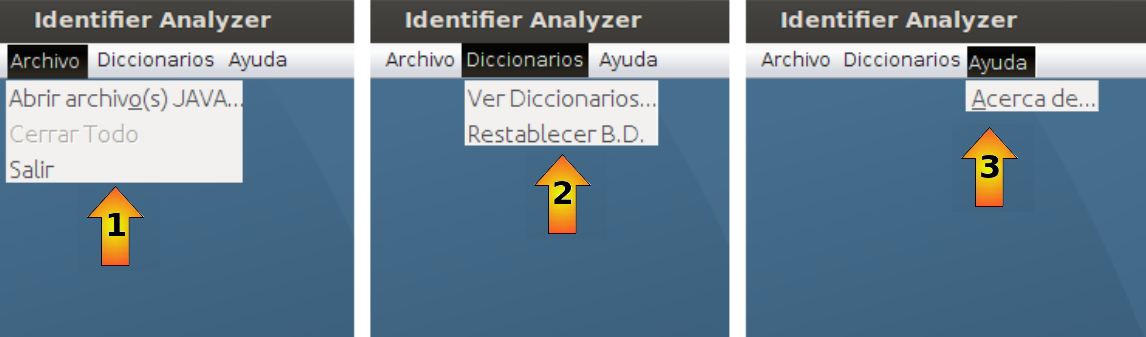
\includegraphics[scale= 0.46]{./cap4/ida_01.png}
}
\caption{Barra de Menú de IDA}
\label{ida1}
\end{figure}

Al pulsar\footnote[1]{El término `pulsar' o `presionar' se utilizará a lo largo del capítulo, significa hacer click con el puntero del ratón.} en \textit{Archivo} de la barra antedicha, se despliega un menú con los siguientes ítems (ver figura \ref{ida1} - Flecha 1):

\begin{description}
\itemsep0em%reduce espacio
\item[Abrir archivo(s) JAVA:] Abre una ventana que permite elegir uno o varios archivos con extensión JAVA (ver figura \ref{ida2}). Los archivos seleccionados serán analizados por IDA (en la próxima sección, serán dados más detalles).
\item[Cerrar Todo:] Cierra todos los archivos JAVA abiertos actualmente en la aplicación.
\item[Salir:] Cierra la Aplicación.
\end{description}

Cuando se pulsa en \textit{Diccionarios} de la barra de menú, se despliega otro menú con con los siguientes ítems (ver figura \ref{ida1} - Flecha 2):

\begin{description}
\itemsep0em%reduce espacio

\item[Ver Diccionarios:] Abre una ventana, que muestra un listado de palabras en Inglés correspondiente al diccionario \textit{ispell} (explicado en la sección anterior). %\footnote[1]{Comando de Linux generalmente utilizado para corregir errores ortográficos (inglés) en archivos de texto. http://wordlist.aspell.net}. 
La ventana antedicha, también muestra un listado de palabras irrelevantes o stoplist (explicado en la sección anterior). Esta ventana, se explica con más detalles en la sección \ref{sec:panPalDicc}.

\item[Restablecer B.D.(Base de Datos):] Genera nuevamente la base de datos HSQLDB. En caso de haber problemas con la base de datos, es útil restablecerla.

%Esta regeneración toma datos de los archivos ubicados en la carpeta `Diccionarios' dentro del proyecto de la herramienta IDA. Restablecer la base es útil cuando se agregan nuevos datos a los diccionarios desde los archivos previamente descriptos.
\end{description}

Finalmente al presionar \textit{Ayuda} de la barra de menú, se despliega un solo botón (ver figura \ref{ida1} - Flecha 3):

\begin{description}
\itemsep0em%reduce espacio
\item[Acerca de:] Brinda información sobre el autor y directores involucrados en la construcción de la herramienta IDA.
\end{description}

\begin{figure}[t] %[h] para here [b] para bottom [t] para top
\centerline{%queda centrada mejor la imagen
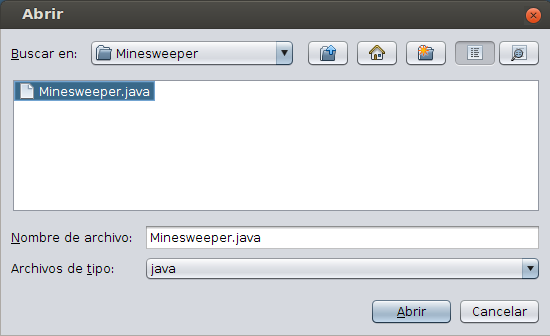
\includegraphics[scale= 0.7]{./cap4/ida_02.png}
}
\caption{Ventana para seleccionar Archivos JAVA.}
\label{ida2}
\end{figure}

\vspace{-1em}

\subsection{Lectura de Archivos JAVA}

Cuando se pulsa en el botón \textit{Abrir archivo(s) JAVA}, (ver figura \ref{ida1} - Flecha 1), se despliega una ventana para que el usuario elija uno o varios archivos JAVA (ver figura \ref{ida2}). 

%Para que IDA funcione correctamente el archivo de entrada JAVA debe cumplir con ciertas validaciones. Una de ellas es, que el código no contenga errores sintácticos (un ejemplo, entre tantos, de error sintáctico es: no colocar punto y coma al final de una sentencia).

Una vez que el usuario elige el/los archivo/s, IDA utiliza un  programa externo llamado JACOBE\footnote[1]{http://www.tiobe.com/jacobe}. Este programa JACOBE, recibe como entrada un archivo JAVA y embellece el código fuente que esta contenido en el. Este embellecimiento se realiza para facilitar la lectura del código al usuario. En la próxima sección se describe el panel que IDA tiene para visualizar el código leído del archivo.

%Si algún archivo de entrada esta vacío o posee algún error sintáctico, JACOBE lo detecta y automáticamente IDA muestra un cartel informando al usuario (ver figura \ref{idaWar1}). 

La herramienta IDA, además realiza un control de los archivos abiertos, impidiendo que se abra el mismo archivo más de una vez. En caso de que esto suceda, se muestra un cartel informando al usuario (ver figura \ref{idaWar2}). Este control se realiza por cuestiones de coherencia al momento de analizar los archivos.

%\begin{figure}[t] %[h] para here [b] para bottom [t] para top
%\centerline{%queda centrada mejor la imagen
%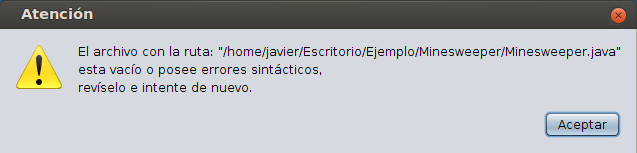
\includegraphics[scale= 0.8]{./cap4/ida_war_01.png}
%}
%\caption{Aviso sobre Archivo JAVA no válido.}
%\label{idaWar1}
%\end{figure}

\begin{figure}[t] %[h] para here [b] para bottom [t] para top
\centerline{%queda centrada mejor la imagen
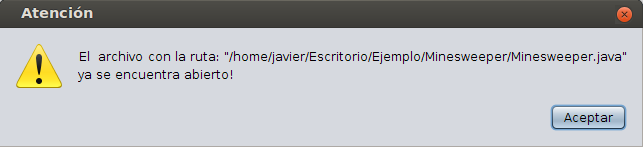
\includegraphics[scale= 0.8]{./cap4/ida_war_02.png}
}
\caption{Aviso sobre Archivo JAVA ya abierto en IDA.}
\label{idaWar2}
\end{figure}

\subsection{Panel de Elementos Capturados}

Después que el programa JACOBE embellece el código contenido en el archivo JAVA,
%si estos cumplen con las validaciones descriptas en la sección anterior, 
el mismo se procesa por el AS explicado en secciones previas. Luego que el AS termina sus tareas de extracción de elementos (ids, comentarios y literales), el \textit{Panel de Elementos Capturados} aparece (ver figura \ref{ida3}). Este panel en la parte superior posee pestañas, cada pestaña posee un rótulo con el nombre del archivo que está siendo analizado (ver figura \ref{ida3} - Flecha 1). Es posible elegir de a varios archivos para analizar, mediante la ventana de selección de archivos (ver figura \ref{ida2}), o también se puede ir eligiendo de a un archivo por apertura de esta ventana.  En caso de querer finalizar el análisis de un archivo particular y cerrar la pestaña, se puede pulsar en la cruz ubicada al lado del rótulo de cada pestaña (ver figura \ref{ida3} - Flecha 1).

\begin{figure}[t!] %[h] para here [b] para bottom [t] para top
\centerline{%queda centrada mejor la imagen
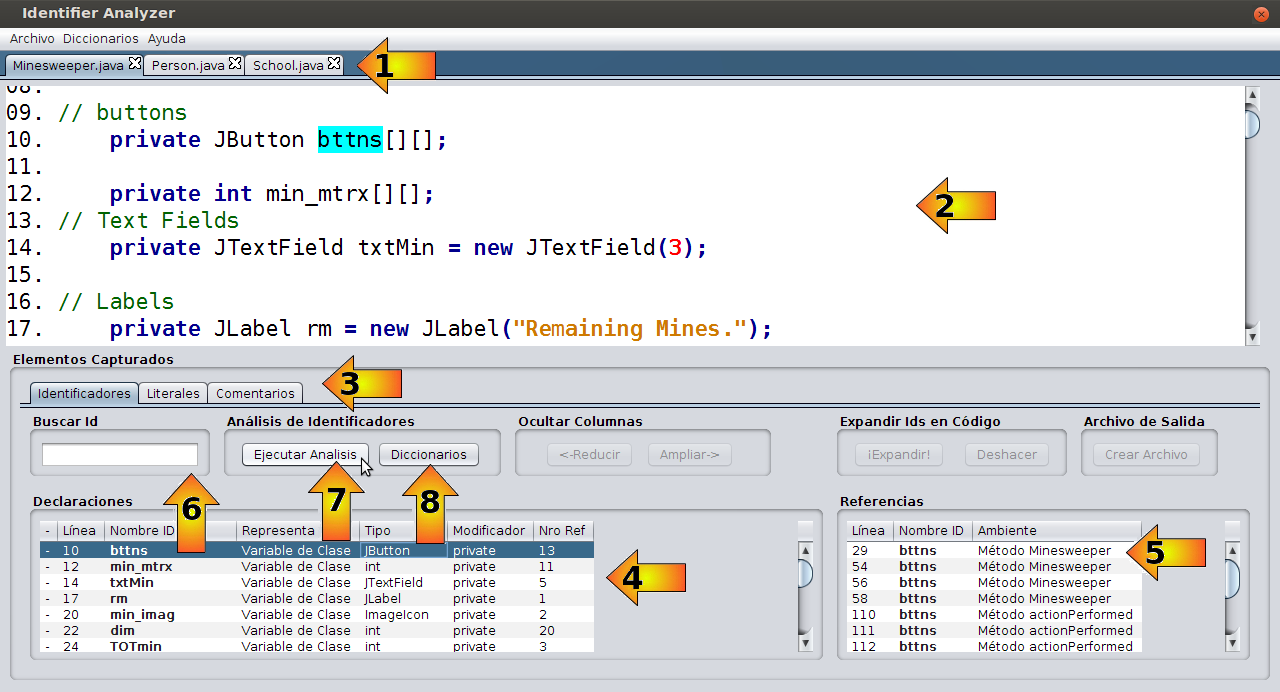
\includegraphics[scale= 0.42]{./cap4/ida_03.png}
}
\caption{Panel de Elementos Capturados}
\label{ida3}
\end{figure}

\begin{figure}[h!] %[h] para here [b] para bottom [t] para top
\centerline{%queda centrada mejor la imagen
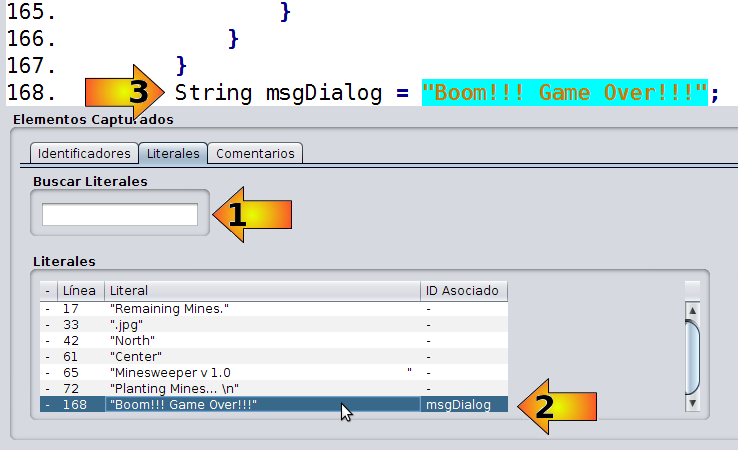
\includegraphics[scale= 0.5]{./cap4/ida_04.png}
}
\caption{Literales Capturados}
\label{ida4}
\end{figure}

Cada pestaña en su interior posee el mismo subpanel que se divide en dos partes principales. La parte superior contiene el código leído y embellecido (por JACOBE) del archivo JAVA (ver figura \ref{ida3} - Flecha 2).
%, el código aquí se presenta ya alineado en su formato por JACOBE. duda
La parte inferior, muestra toda la información extraída por el AS referente a ids, literales y comentarios. Estos últimos tres poseen una pestaña cada uno (ver figura \ref{ida3} - Flecha 3). Al pulsar sobre cada pestaña, se muestra la información clasificada correspondiente (a ids, literales y comentarios), a continuación se describe como se exhibe esta información.

\noindent \textbf{\\\\Pestaña de Identificadores Capturados\\} 

Al pulsar la \textit{Pestaña de Identificadores} (ver figura \ref{ida3} - Flecha 3), se muestra la \textit{Tabla de Declaraciones} (ver figura \ref{ida3} - Flecha 4). Esta tabla enumera los ids capturados por el AS y cada columna se corresponde a: el número de línea donde esta declarado el id, el nombre del id, el tipo (int, char, etc.), el modificador (publico, privado, protegido), lo que el id representa (variable de clase, constructor, método de clase, etc.).
Esta \textit{Tabla de Declaraciones} si se presiona sobre una fila, inmediatamente se resalta con color en el código ubicado en la parte superior, la declaración del id correspondiente (ver figura \ref{ida3} - Flecha 2). 
%Es el mismo comportamiento que tienen las tablas de literales y comentarios explicados anteriormente. 
Cabe destacar que si el usuario lo desea, puede realizar búsquedas en la \textit{Tabla de Declaraciones} por nombre de id; para realizar las estas búsquedas se debe escribir en el cuadro de texto ubicado dentro del recuadro \textit{Buscar Id} (ver figura \ref{ida3} - Flecha 5), a medida que se escriba en este cuadro de texto, se irán filtrando los resultados en la \textit{Tabla de Declaraciones}.

\begin{figure}[t] %[h] para here [b] para bottom [t] para top
\centerline{%queda centrada mejor la imagen
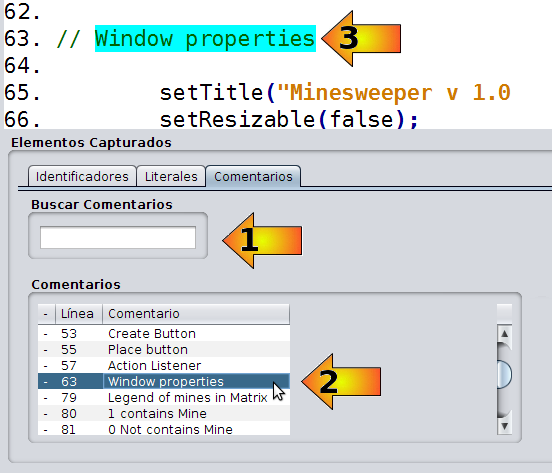
\includegraphics[scale= 0.55]{./cap4/ida_05.png}
}
\caption{Comentarios Capturados}
\label{ida5}
\end{figure}

\noindent \textbf{\\Pestaña de Literales Capturados\\} 

Al pulsar la \textit{Pestaña de Literales} (ver figura \ref{ida3} - Flecha 3), se puede apreciar que aparece una \textit{Tabla de Literales} y un práctico buscador en forma de cuadro de texto (ver figura \ref{ida4} - Flecha 1 y 2). Esta tabla contiene dos columnas, número de línea del literal y el literal propiamente dicho (ver figura \ref{ida4} - Flecha 2).
De manera similar a la que se describió en el párrafo precedente, el buscador filtra los resultados en la \textit{Tabla de Literales} mientras se va escribiendo en el. También al pulsar sobre alguna fila, automáticamente el literal correspondiente se resalta en el código que está ubicado en la parte superior (ver figura \ref{ida4} - Flecha 3).

\noindent \textbf{\\Pestaña de Comentarios Capturados\\} 

De manera equivalente, al presionar la \textit{Pestaña de Comentarios} (ver figura \ref{ida3} - Flecha 3), se visualiza la \textit{Tabla de Comentarios} y un buscador de comentarios en esta tabla (ver figura \ref{ida5} - Flecha 1). La \textit{Tabla de Comentarios} posee dos columnas que corresponden, por un lado al comentario y por el otro al número de línea donde se encuentra el comentario dentro del código (ver figura \ref{ida5} - Flecha 2). Al igual que se describió en el párrafo anterior, al presionar en una de las filas de la \textit{Tabla de Comentarios} inmediatamente se resalta en el código de la parte superior, la ubicación del comentario seleccionado (ver figura \ref{ida5} - Flecha 3).\\

Hasta aquí, solo se ha descripto como IDA exhibe la información útil que fue capturada del código por el AS. A continuación, se explicará como se emplea IDA para analizar los ids. Para ello, se debe pulsar en la \textit{Pestaña de Identificadores} (ver figura \ref{ida3} - Flecha 3), luego pulsar en el botón \textit{Ejecutar Análisis} ubicado dentro del cuadro \textit{Análisis de Identificadores} (ver figura \ref{ida3} - Flecha 6), al hacerlo se abrirá la \textit{Ventana de Análisis} que será explicada en la próxima sección.

\begin{figure}[h!] %[h] para here [b] para bottom [t] para top
\centerline{%queda centrada mejor la imagen
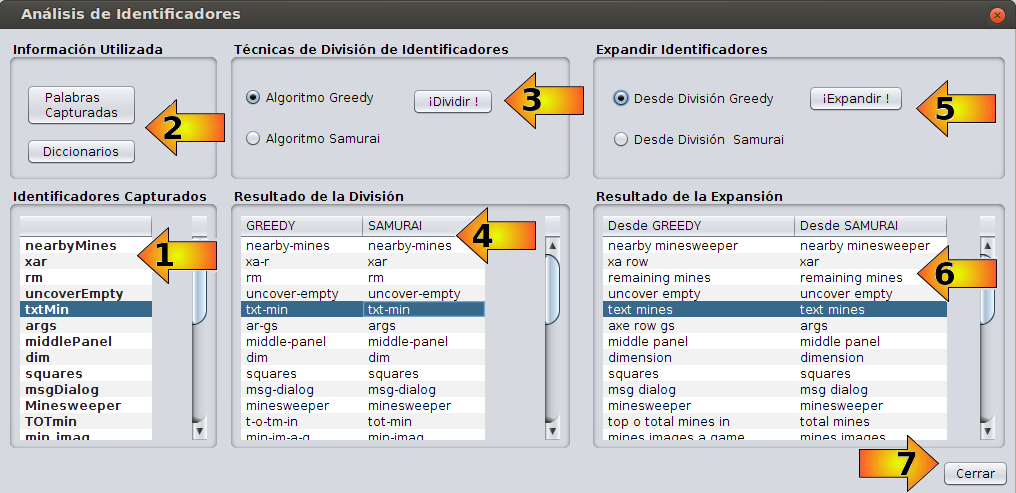
\includegraphics[scale= 0.52]{./cap4/ida_06.png}
}
\caption{Ventana de Análisis}
\label{ida6}
\end{figure}

\subsection{Ventana de Análisis}

La \textit{Ventana de Análisis} (ver figura \ref{ida6}) contiene 3 partes principales, (de izquierda a derecha):

\begin{description}

\item[Parte Izquierda:] Posee un listado con los ids capturados, en el cuadro inferior izquierdo (ver figura \ref{ida6} - Flecha 1). Arriba de estos se encuentran dos botones \textit{Palabras Capturadas} y \textit{Diccionarios} (ver figura \ref{ida6} - Flecha 2), al pulsarlos le brindan información al usuario sobre los datos que se utilizan para ejecutar los algoritmos de análisis, y ambos botones serán explicados con más detalles en la próxima sección.

\item[Parte Central:] Ubicado en la parte central, en el cuadro superior (ver figura \ref{ida6} - Flecha 3) se pueden seleccionar los dos algoritmos de división de ids (Greedy y Samurai), el botón \textit{Dividir} del mismo cuadro ejecuta el algoritmo seleccionado. Los resultados obtenidos se muestran en el cuadro central inferior, en una tabla con los resultados. En la figura \ref{ida6} - Flecha 4 se muestran ambas técnicas (Greedy y Samurai) ya ejecutadas y enumerando los resultados.

\item[Parte Derecha:] Al presionar el botón \textit{Expandir}, situado en el cuadro superior derecho (ver figura \ref{ida6} - Flecha 5), ejecuta el algoritmo de expansión básico tomando como entrada los ids divididos desde Greedy o desde Samurai, según haya seleccionado el usuario en este mismo cuadro (ver figura \ref{ida6} - Flecha 5). Los resultados obtenidos de las expansiones (desde Greedy y desde Samurai), se muestran en la tabla situada en el cuadro inferior derecho. En la figura \ref{ida6} - Flecha 6 se pueden apreciar las expansiones realizadas.

\end{description}

\begin{figure}[t] %[h] para here [b] para bottom [t] para top
\centerline{%queda centrada mejor la imagen
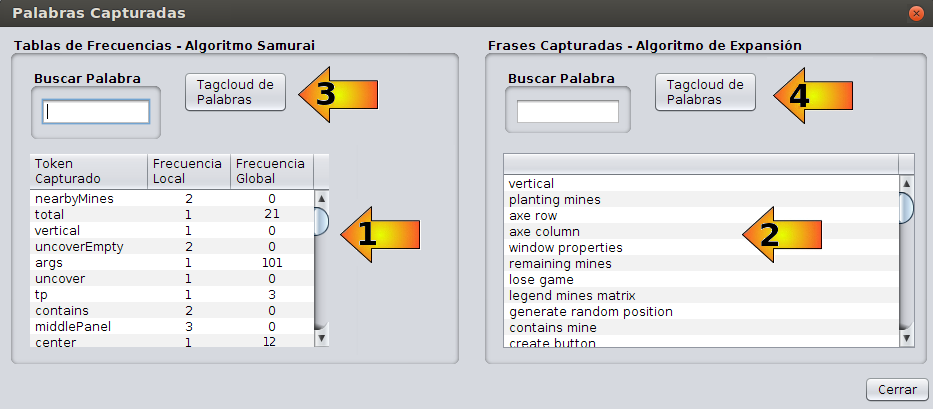
\includegraphics[scale= 0.55]{./cap4/ida_07.png}
}
\caption{Información Utilizada para el Análisis de Ids}
\label{ida7}
\end{figure}

\subsection{Palabras Capturadas y Diccionarios}
\label{sec:panPalDicc}

En la sección anterior, se nombraron dos botones \textit{Palabras Capturadas} y \textit{Diccionarios}, ubicados en la \textit{Ventana de Análisis} (ver figura \ref{ida6} - Flecha 2). A continuación, se describirán la función de cada uno de ellos.

\noindent \textbf{\\Ventana de Palabras Capturadas\\} 

Al pulsar el botón \textit{Palabras Capturadas}, se abre una ventana que posee dos cuadros (ver figura \ref{ida7}), el cuadro de la izquierda contiene una tabla que muestra las frecuencias correspondiente al Algoritmo Samurai (ver figura \ref{ida7} - Flecha 1). Esta tabla tiene tres columnas, en la primera posee tokens\footnote[1]{El concepto “token” se asocia a palabras que están contenidas en literales, comentarios e ids, este último necesita un proceso especial, para más detalles ver cap. 3 - sección \ref{sec:algSamu}}, los mismos fueron capturados por el AS ANTLR. La segunda columna, contiene la frecuencia local de cada token, cabe recordar que la frecuencia local se construye en función de la frecuencia absoluta de aparición de los tokens en el código del archivo actual. La tercera y última columna de la tabla denota la frecuencia global de cada token, la misma esta predefinida en la base de datos HSQLDB (ver sección \ref{sec:bseEmb}).

El cuadro de la derecha, lista en una tabla las frases capturadas (ver figura \ref{ida7} - Flecha 2), estas frases se obtienen de los comentarios y los literales strings, el Algoritmo de Expansión es el encargado de utilizarlas (ver capítulo 3 - sección \ref{sec:algExpBas}). Este algoritmo las usa, ya que estas frases son posibles candidatas a expandir las abreviaturas en forma de acrónimo que puede contener un id (Ejemplo: \textsf{fl} $\rightarrow$ \textsf{file system}).

A modo de agilizar las búsquedas en las tablas descriptas anteriormente (la de frecuencias de Samurai y la de frases), se puede llevar a cabo utilizando los cuadros de texto con rótulo \textit{Buscar Palabra} situados al lado de cada botón \textit{TagCloud de Palabras} (ver figura \ref{ida7} - Flechas 3 y 4).

\begin{figure}[t] %[h] para here [b] para bottom [t] para top
\centerline{%queda centrada mejor la imagen
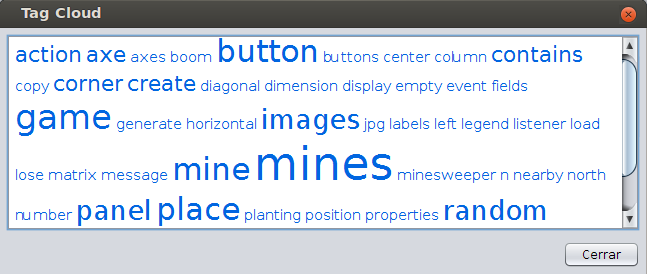
\includegraphics[scale= 0.75]{./cap4/ida_08.png}
}
\caption{TagCloud: Nube de Etiquetas}
\label{ida8}
\end{figure}

\noindent \textbf{\\Ventana de TagCloud (Nube de Etiquetas)\\} 

Como se puede observar en la figura \ref{ida7} - Flechas 3 y 4, existen dos botones con el nombre de \textit{TagCloud de Palabras}, cada uno abre una ventana que contiene una \textit{Nube de Etiquetas} (ver figura \ref{ida8}). Esta nube posee palabras y resalta en tamaño más grande aquellas palabras que más frecuencia de aparición tienen (En la figura \ref{ida8} las palabras \textsf{mine}, \textsf{mines}, \textsf{game} etc. son las que mayor aparición tienen). Para generar esta nube se emplea una librería de JAVA llamada OpenCloud\footnote[1]{http://opencloud.mcavallo.org}.
Esta \textit{Nube de Etiquetas} ayuda a ver con más claridad que palabras son más frecuentes en el código. 

Para el caso de la nube de frecuencias de Samurai (ver figura \ref{ida7} - Flecha 3), el tamaño de cada palabra depende de la Frecuencia Local de cada token (ver figura \ref{ida7} - Flecha 1). En el caso de la nube de las frases capturadas (ver figura \ref{ida7} - Flecha 4), el tamaño de las palabras esta dado por el número de apariciones dentro de esta tabla de frases (ver figura \ref{ida7} - Flecha 2).

\begin{figure}[t] %[h] para here [b] para bottom [t] para top
\centerline{%queda centrada mejor la imagen
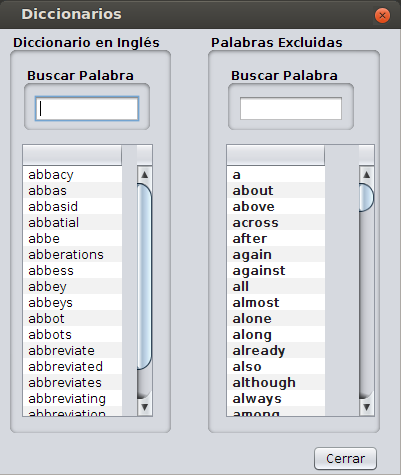
\includegraphics[scale= 0.58]{./cap4/ida_09.png}
}
\caption{Ventana de Diccionarios}
\label{ida9}
\end{figure}

\noindent \textbf{\\Ventana de Diccionarios\\} 

Volviendo a la \textit{Ventana de Análisis} si se pulsa el botón \textit{Diccionarios} (ver figura \ref{ida6} - Flecha 2), se abre la \textit{Ventana de Diccionarios} (ver figura \ref{ida9}). Esta ventana posee dos tablas, la tabla de la izquierda lista todas las palabras en inglés que tiene el diccionario del comando de Linux \textit{ispell}, esta lista de palabras es utilizada por el Algoritmo Greedy y el Algoritmo Expansión Básica (ver sección \ref{sec:bseEmb} de este capítulo). La segunda tabla de la derecha enumera las palabras que pertenecen a la stoplist o lista de palabras irrelevantes, también utilizada por los dos algoritmos antedichos. Convenientemente, ambas tablas poseen un buscador por palabras dado que el contenido de cada una es amplio (ver figura \ref{ida9}). Esta \textit{Ventana de Diccionarios} puede ser invocada desde otros lugares de la herramienta IDA. Uno de ellos es desde la barra de menú (ver Figura \ref{ida1} - Flecha 2). Otro sitio donde puede abrirse, es desde el \textit{Panel de Elementos Capturados}, pulsando el botón que esta al lado de \textit{Ejecutar Análisis} (ver figura \ref{ida3} - Flecha 7).

Todas las ventanas que fueron descriptas previamente (palabras capturadas, tagcloud, diccionarios), en caso de haber sido abiertas por el usuario, el mismo debe cerrarlas si desea continuar con el proceso de análisis de ids.

\begin{figure}[t!] %[h] para here [b] para bottom [t] para top
\centerline{%queda centrada mejor la imagen
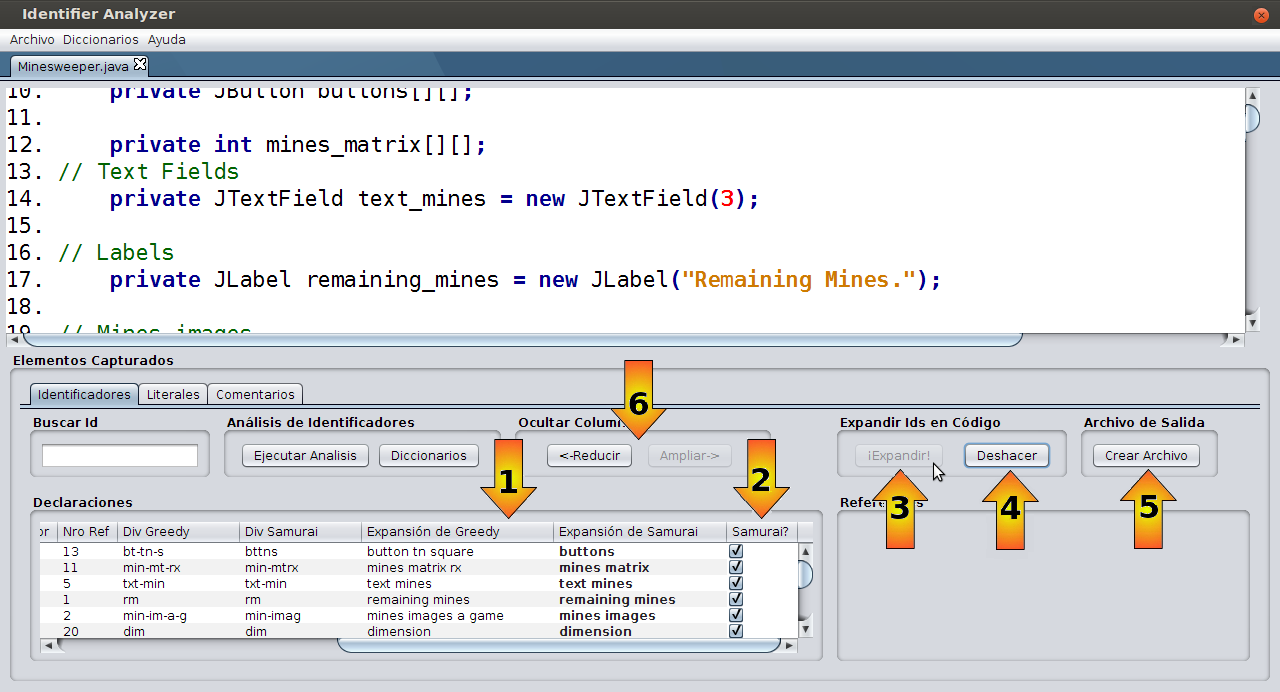
\includegraphics[scale= 0.42]{./cap4/ida_10.png}
}
\caption{Panel de Elementos Capturados}
\label{ida10}
\end{figure}


\begin{figure}[t] %[h] para here [b] para bottom [t] para top
\centerline{%queda centrada mejor la imagen
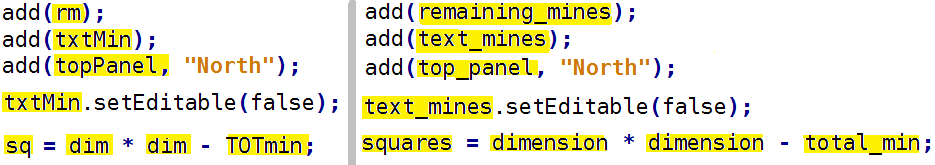
\includegraphics[scale= 0.63]{./cap4/ida_11.png}
}
\caption{Tabla del Análisis de Ids en Navegador Web.}
\label{ida11}
\end{figure}

\subsection{Nuevamente al Panel de Elementos Capturados}

Una vez que los ids fueron analizados (Divididos y Expandidos) mediante la \textit{Ventana de Análisis}, la misma debe ser cerrada presionando el botón \textit{Cerrar} (ver figura \ref{ida6} - Flecha 7). Esta acción, retorna al \textit{Panel de Elementos Capturados} nuevamente (ver figura \ref{ida10}).
Como se puede observar, en la tabla \textit{Declaraciones} que detalla los ids extraídos e información asociada a estos, se le suman nuevas columnas (ver figura \ref{ida10} - Flecha 1). Estas nuevas columnas contienen los resultados obtenidos de los algoritmos de división (Greedy, Samurai) y el algoritmo de expansión ejecutados en la \textit{Ventana de Análisis}; las columnas nuevas son: División Greedy, División Samurai, Expansión desde Greedy y Expansión desde Samurai.

Al agregar las columnas nuevas se habilita el cuadro \textit{Ocultar Columnas}. En el se encuentran dos botones \textit{Reducir} y \textit{Ampliar} (ver figura \ref{ida10} - Flecha 2). El primero de ellos a modo de facilitar la visualización, oculta las columnas que hay entre los ids y las columnas que contienen el análisis de ids (las columnas que se ocultan son: tipo, modificador, Representa), de esta manera el usuario puede comparar más claramente las distintas divisiones y expansiones de ids. Mientras que el botón \textit{Ampliar} restablece las columnas originales.

%Cuando el usuario termina de seleccionar la mejor expansión de cada id, se procede al cuadro \textit{Expandir Ids en Código}. Este cuadro contiene dos botones, al presionar \textit{Expandir} (ver figura \ref{ida10} - Flecha 3), la herramienta IDA reemplaza los ids del código de acuerdo a lo seleccionado en las casillas de selección en la tabla de \textit{Declaraciones} que fue explicado al principio de esta sección.
%Una vez realizado esto, el código es más comprensivo para el usuario, en la figura \ref{ida11} se puede observar dos trozos de códigos, el de la arriba se observa el código normal, mientras que el de la abajo posee los ids expandidos.
%En caso de querer retrotraer la acción de reemplazo de ids, se puede pulsar en el botón \textit{Deshacer} ubicado también en el cuadro \textit{Expandir Ids en Código} (ver figura \ref{ida10} - Flecha 4) y restablecer el código original.

Luego si el usuario lo decide, puede presionar el botón \textit{Abrir} en el cuadro \textit{Ver Tabla en Navegador} (ver figura \ref{ida10} - Flecha 3). Esta acción abre automáticamente el navegador web por defecto del sistema operativo, y mediante una pagina web en formato html, se muestra una tabla con los resultados obtenidos producto del análisis de ids (ver figura \ref{ida11}). De esta manera, el usuario puede visualizar más claramente el análisis realizado, permitiendo también imprimir los resultados en papel (mediante el navegador web), si el usuario lo desea.

Dando como finalizado el proceso necesario que debe realizar el usuario para analizar los ids con la herramienta IDA, en la próxima sección se explican los casos de estudios realizados que demuestran la utilidad de IDA.

\pagebreak
\section{Casos de Estudio}

En esta sección se presentarán 3 casos de estudios realizados con la herramienta IDA. En cada uno de estos casos, se examinan los ids de un único archivo JAVA. A través de tablas, se irán mostrando los resultados parciales que se van obteniendo durante el proceso de análisis de los ids.
Con estos casos, se pretende ostentar la utilidad de la herramienta IDA en lo que respecta al análisis de ids y mostrar que es un aporte al área de la CP.

\subsection{Buscaminas (Minesweeper)}

El programa JAVA denominado Minesweeper.java, al ejecutarlo posee el clásico y conocido juego llamado Buscaminas (Minesweeper en Inglés - ver figura \ref{caso1}). Este programa contiene un módulo de 250 líneas aproximadamente que fueron analizadas por IDA.

Al ingresarse el programa Minesweeper.java a la herramienta IDA, se da comienzo a la fase de extracción de datos y el analizador sintáctico captura información referente a los ids. Esta información la exhibe IDA al usuario en el \textit{Panel de Elementos Capturados}, en la tabla \textit{Declaraciones} (ver figura \ref{ida3} - flecha 4). En la tabla \ref{tabla2} se puede apreciar esta información: la línea donde esta declarado el id, que representa en el código analizado, el tipo, el modificador .

\begin{figure}[t] %[h] para here [b] para bottom [t] para top
\centerline{%queda centrada mejor la imagen
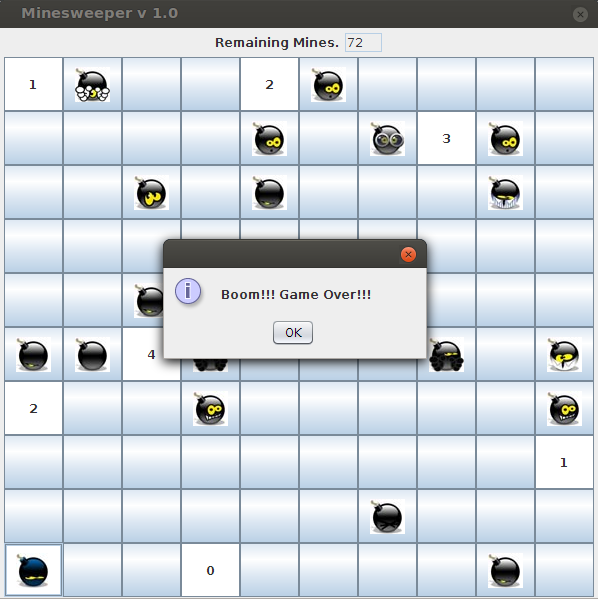
\includegraphics[scale= 0.6]{./cap4/caso_01.png}
}
\caption{Captura del Juego Buscaminas programado en JAVA}
\label{caso1}
\end{figure}


Para hacer una descripción más detallada sobre los ids capturados, en la tabla \ref{tabla2} se puede observar que el archivo \mbox{Minesweeper.java}
tiene ids del tipo \textit{hardwords} y \textit{softwords} (ver capítulo 3). Algunos \textit{hardwords} que se pueden observar son \textsf{min\_mtrx}, \textsf{TOTmin}, \textsf{topPanel} (entre otros), ya que estos poseen una marca de separación que destacan las palabras que lo componen. Por otro lado, algunos de los \textit{softwords} que se capturaron son \textsf{ae}, \textsf{plantmines}, \textsf{bttns} (entre otros).



A su vez, se capturaron los comentarios junto a la línea del código donde se ubican cada uno, los mismos se muestran en tabla \ref{tabla3}. De la misma forma, los literales Strings que se extrajeron se exhiben en la tabla \ref{tabla4}. En esta tabla, se puede observar que además del número de línea donde se ubica el literal. 
Tanto los literales y los comentarios se visualizan en IDA a través del \textit{Panel de Elementos Capturados}, eligiendo la pestaña correspondiente (ver figura \ref{ida3} - Flecha 3).

Es importante recordar, que los comentarios y literales de las tablas \ref{tabla3} y \ref{tabla4} son usados para construir la lista de frases que se muestra en la ventana de \textit{Palabras Capturadas} en la figura \ref{ida7} - flecha 4. Esta información es útil para el Algoritmo de Expansión.

A continuación, se procede a analizar los ids, el usuario realiza esto con la \textit{Ventana de Análisis} (ver figura \ref{ida6}) aplicando las técnicas de división (Greedy y Samurai) y después la técnica de expansión de abreviaturas. Los resultados más destacados se pueden apreciar en la tabla \ref{tabla5}.

\pagebreak

\noindent \textbf{Análisis de Resultados\\}

La información mostrada en la tabla \ref{tabla5}, las columnas de \textit{Greedy} y \textit{Samurai} muestran los resultados de división de dichos Algoritmos. En las columnas \textit{Expansión desde Greedy} y \textit{Expansión desde Samurai} se enumeran los resultados de haber expandido las distintas partes del id, que resultaron desde los Algoritmos Greedy y Samurai respectivamente.

Los ids analizados por la herramienta IDA (ver tabla \ref{tabla5}) en lo que respecta a \textit{hardwords}, se pueden encontrar con guión bajo  \textsf{min\_imag}, \textsf{min\_mtrx}  para el tipo camel-case  \textsf{uncoverEmpty}, \mbox{\textsf{msgDialog}} y para el caso especial \textsf{TOTmin}, \textsf{MINSnum} (variante camel-case), entre otros. El algoritmo Greedy manifiesta irregularidades a la hora de dividir ya que siempre considera que la mayor cantidad de divisiones es la mejor opción, esto puede observarse en casos como \textsf{min--im--ag},  \textsf{bt--tn--s}, \textsf{min--sn--um} (ver tabla \ref{tabla5} - columna Greedy). Para el caso especial \textsf{MINSnum}, es interesante observar como Samurai se da cuenta de donde hacer la división, y no la considera un caso común de camel-case que la separa antes de la mayúscula seguido de minúscula (ver capítulo 3). No sucediendo lo mismo que Greedy ya supone que es del tipo camel-case haciendo la separación incorrecta \textsf{min--sn--um}.

En lo que respecta a softwords se aprecia la presencia de acrónimos como \textsf{rm} y \textsf{ae} (entre otros). El Algoritmo de Expansión consulta la lista de frases (ver figura \ref{ida7} - flecha 4) conformada por comentarios y los literales capturados (ver tablas \ref{tabla3} y \ref{tabla2}), al encontrar coincidencia con el literal \textsf{“remaining mines”} y el comentario \textsf{“action event”}, selecciona ambos como la expansión correspondiente de \textsf{rm} y \textsf{ae} (ver tabla \ref{tabla5} - Columnas de Expansión).
El resto de los softwords se puede considerar a \textsf{mins}, \textsf{bttns}, \textsf{dim}, aquí Greedy también acusa inconvenientes separando los ids, mientras que Samurai no los divide (ver tabla \ref{tabla5}). %falta mostrar las tablas de frecuencias

Para finalizar, los ids  \textsf{i}, \textsf{j} son comunes en la mayoría de los códigos, y son difíciles de traducir. Por ende, el Algoritmo de Expansión busca en las tablas de Literales y Comentarios  (ver tablas \ref{tabla3} y \ref{tabla4}), palabras que estén dentro del \textit{Dominio del Problema} y de esta manera tratar de darle una traducción válida en este contexto.

\begin{sidewaystable}[h!]
\centering
	\begin{tabular}{| c | c | c | c | c |}      
       \hline
  	   \textbf{Línea} & \textbf{Nombre ID} & \textbf{Representa} & \textbf{Tipo} & \textbf{Modificador} \\ \hline
7&Minesweeper&Clase&--&public \\ \hline
10&bttns&Variable de Clase&JButton&private \\ \hline
12&min\_mtrx&Variable de Clase&int&private \\ \hline
14&txtMin&Variable de Clase&JTextField&private \\ \hline
17&rm&Variable de Clase&JLabel&private \\ \hline
20&min\_imag&Variable de Clase&ImageIcon&private \\ \hline
22&dim&Variable de Clase&int&private \\ \hline
24&TOTmin&Variable de Clase&int&private \\ \hline
25&sq&Variable de Clase&int&private \\ \hline
%28&Minesweeper&Constructor&--&public \\ \hline
37&topPanel&Variable Local&JPanel&-- \\ \hline
48&middlePanel&Variable Local&JPanel&-- \\ \hline
71&plantmines&Método de Clase&void&private \\ \hline
71&mins&Parámetro&int&-- \\ \hline
102&main&Método de Clase&void&public \\ \hline
102&args&Parámetro&String[]&-- \\ \hline
107&actionPerformed&Método de Clase&void&public \\ \hline
107&ae&Parámetro&ActionEvent&-- \\ \hline
124&uncoverEmpty&Método de Clase&void&private \\ \hline
124&j&Parámetro&int&-- \\ \hline
124&i&Parámetro&int&-- \\ \hline
%134&restart&Método de Clase&void&private \\ \hline
150&win&Método de Clase&void&private \\ \hline
159&boom&Método de Clase&void&private \\ \hline
172&msgDialog&Variable Local&String&-- \\ \hline
179&nearbyMines&Método de Clase&int&private \\ \hline
188&MINSnum&Variable Local&int&-- \\ \hline
179&xar&Parámetro&int&-- \\ \hline
179&yac&Parámetro&int&-- \\ \hline
   
   	\end{tabular}  
	 
   \caption{Identificadores extraídos por el AS ANTLR}
   \label{tabla2}
     
\end{sidewaystable} 


\begin{table}[ht!]
\parbox{.40\linewidth}{
 
		\centering
   		\begin{tabular}{| c | c |}  
       \hline
\textbf{Línea} & \textbf{Comentario} \\ \hline
9&buttons  \\ \hline
13&Text Fields  \\ \hline
16&Labels  \\ \hline
19&Mines images  \\ \hline
21&Dimension  \\ \hline
23&total mines  \\ \hline
27&Time tp  \\ \hline
31&load Images  \\ \hline
36&Top Panel  \\ \hline
47&Button panel  \\ \hline
50&Create and place button  \\ \hline
53&Create Button  \\ \hline
55&Place button  \\ \hline
57&Action Listener  \\ \hline
63&Window properties  \\ \hline
80&Legend of mines in Matrix  \\ \hline
81&1 contains Mine  \\ \hline
82&0 Not contains Mine  \\ \hline
83&Place random mine  \\ \hline
\end{tabular}
}
\hfill
\parbox{.48\linewidth}{
 
		\centering
   		\begin{tabular}{| c | c |}  
       \hline
\textbf{Línea} & \textbf{Comentario} \\ \hline
85&Generate random position \\ \hline
91&Place mine \\ \hline
93&Display mines panel \\ \hline
107&Action Event \\ \hline
126&Uncover an empty square \\ \hline
129&Nearby Mines \\ \hline
136&restart game \\ \hline
152&Win the game \\ \hline
161&lose the game \\ \hline
165&Mines Random Images \\ \hline
183&x axe row \\ \hline
184&y axe column \\ \hline
186&return the number of mines \\ \hline
192&horizontal \\ \hline
199&vertical \\ \hline
207&diagonal \\ \hline
208&Top left corner \\ \hline
209&copy of axes \\ \hline
224&top right corner \\ \hline
\end{tabular}
}
\caption{Comentarios extraídos por el AS ANTLR}\label{tabla3}
\end{table}


\begin{table}[h!]
	
		\centering
   		\begin{tabular}{| c | c |}      
       \hline
  	   \textbf{Línea} & \textbf{Literal} \\ \hline
17&“Remaining Mines.” \\ \hline
33&“.jpg”  \\ \hline
42&“North”  \\ \hline
61&“Center”  \\ \hline
65&“Minesweeper v 1.0 ”  \\ \hline
73&“Planting Mines...”  \\ \hline
153&“You Win!!! Game Over!!!” \\ \hline
155&“Message” \\ \hline
173&“Boom!!! Game Over!!!” \\ \hline
175&“Message” \\ \hline
  \end{tabular} 
	 
   \caption{Literales extraídos por el AS ANTLR}
   \label{tabla4}
     
\end{table} 


\begin{sidewaystable}[h!]

		\centering
   		\begin{tabular}{| c | c | c | c | c |}     
   		
       \hline
  	   \textbf{Id} & \textbf{Greedy} & \textbf{Samurai} & \textbf{Exp. desde Greedy} & \textbf{Exp. desde Samurai} \\ \hline
Minesweeper&minesweeper&minesweeper&minesweeper&minesweeper\\ \hline
bttns&bt--tn--s&bttns&button tn square&buttons\\ \hline
min\_mtrx&min--mt--rx&min--mtrx&mines matrix rx&mines matrix\\ \hline
txtMin&txt--min&txt--min&text mines&text mines\\ \hline
rm&rm&rm&remaining mines&remaining mines\\ \hline
min\_imag&min--im--ag&min--imag&mines images ag&mines images\\ \hline
dim&dim&dim&dimension&dimension\\ \hline
TOTmin&tot--min&tot--min&total mines&total mines\\ \hline
sq&sq&sq&square&square\\ \hline
%Minesweeper&minesweeper&minesweeper&minesweeper&minesweeper\\ \hline
topPanel&top--panel&top--panel&top panel&top panel\\ \hline
middlePanel&middle--panel&middle--panel&middle panel&middle panel\\ \hline
plantmines&plant--mines&plant--mines&planting minesweeper&planting minesweeper\\ \hline
mins&min--s&mins&mines square&mines\\ \hline
main&main&main&main&main\\ \hline
args&args&args&args&args\\ \hline
actionPerformed&action--performed&action--performed&action performed&action performed\\ \hline
ae&ae&ae&action event&action event\\ \hline
uncoverEmpty&uncover--empty&uncover--empty&uncover empty&uncover empty\\ \hline
j&j&j&jpg&jpg\\ \hline
i&i&i&images&images\\ \hline
%restart&restart&restart&restart&restart\\ \hline
win&win&win&window&window\\ \hline
%msgDialog&msg--dialog&msg--dialog&message dialog&message dialog\\ \hline
boom&boom&boom&boom&boom\\ \hline
msgDialog&msg--dialog&msg--dialog&message dialog&message dialog\\ \hline
nearbyMines&nearby--mines&nearby--mines&nearby minesweeper&nearby minesweeper\\ \hline
%yac\_cp&y--ac--cp&yac--cp&year action copy&y axe column copy\\ \hline
%xar\_cp&xa--r--cp&xar--cp&xa row copy&x axe row copy\\ \hline
MINSnum&min--sn--um&mins--num&mines sn um&mines number\\ \hline
xar&xa--r&xar&xa row&x axe row\\ \hline
yac&y--ac&yac&yellow action&y axe column\\ \hline

  \end{tabular}
	 
   \caption{Análisis Realizado a los Ids extraídos de Minesweeper.java}
   \label{tabla5}
     
\end{sidewaystable}

\clearpage %esto es necesario sino las tablas se van al final del capitulo

\begin{figure}[t] %[h] para here [b] para bottom [t] para top
\centerline{%queda centrada mejor la imagen
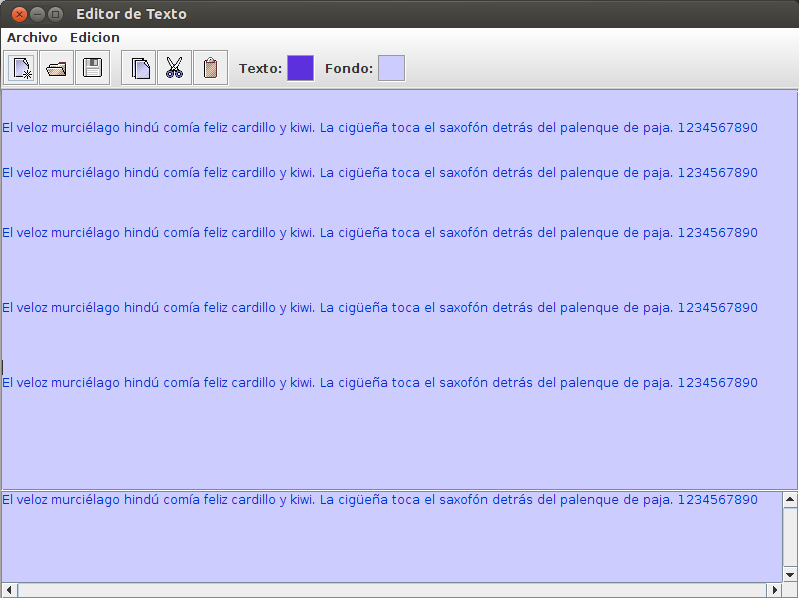
\includegraphics[scale= 0.65]{./cap4/caso_02.png}
}
\caption{Captura del Editor de texto programado en JAVA}
\label{caso2}
\end{figure}

\subsection{Editor de Texto}

Cabe destacar que, a modo de facilitar la lectura, de aquí en adelante, por cada caso de estudio, se mostrará únicamente la tabla con resultados obtenidos producto del análisis de los ids. Se excluyen las tablas de comentarios y literales.

En el próximo caso de estudio, se seleccionó un programa escrito en JAVA que corresponde a un editor de texto (ver figura \ref{caso2}). Este editor posee las herramientas básicas para crear o modificar archivos de textos sin formato, permite cambiar la visualización de colores en las letras y en el fondo, también imprime los archivos que se abran en el.
Este editor esta programado con alrededor de 500 líneas de código, las cuales están escritas en un único archivo llamado Editor.java. 

A continuación, el editor de textos se analiza con la herramienta IDA, el análisis efectuado en los ids se exhibe en la tabla \ref{tabla6}. Dado que este programa posee muchos ids, los resultados que se presentan en la tabla \ref{tabla6} son los más destacados y no son la totalidad.\\

\noindent \textbf{Análisis de Resultados\\}

A simple vista, se puede observar en la tabla \ref{tabla6}, al igual que el caso de estudio de la sección anterior, que las divisiones entre Greedy y Samurai, las de este último son las que mejor se realizan. Esto ocurre por que Greedy siempre selecciona la mayor cantidad de divisiones en la palabra como la mejor opción (ver capítulo 3). Ejemplos de divisiones mal hechas por Greedy son \textsf{bckCol} $\rightarrow$ \textsf{b--c--k--col},
\textsf{btAcept} $\rightarrow$ \textsf{bt--ace--pt}, \textsf{jChoColor} $\rightarrow$ \textsf{j--c--ho--color}, entre otros. 

Sin embargo, en este caso de estudio a diferencia del anterior existen algunas divisiones en las que Samurai falla, los ids que se pueden observar son: \textsf{flreader}, \textsf{ptjob} los cuales no se dividieron como lo hizo Greedy en \mbox{\textsf{fl--reader}}, \textsf{pt--job}. La primer hipótesis que se maneja sobre este resultado, es que Greedy encuentra en el diccionario en Inglés las palabras \textsf{reader} y \textsf{job}. Mientras que Samurai en su función de \textit{Score}, las palabras \textsf{fl} con \textsf{reader} y \textsf{pt} con \textsf{job} no representan puntajes (score) altos para ser divididas entre ellas \mbox{(ver capítulo 3).}

En lo que respecta a la expansión de ids, la mayoría de las abreviaturas resultantes de la división de ids fueron expandidas; algunos ejemplos son \textsf{sel} $\rightarrow$ \textsf{select}, \textsf{tl} $\rightarrow$ \textsf{tool}, \textsf{cl} $\rightarrow$ \textsf{close}, \textsf{bck} $\rightarrow$ \textsf{background}, entre otras. Estas palabras son expandidas por el algoritmo de expansión, gracias a los comentarios y literales capturados por el AS.
Por otro lado, existen algunas abreviaturas que no se expanden como es el caso de \textsf{bt} a \textsf{button}, \textsf{it} a \textsf{item}; que forman parte de los ids \textsf{bt--acept} y \textsf{men--it--new}. La hipótesis de este comportamiento, se debe por que estas abreviaturas son tratadas como acrónimos (abreviaturas que poseen más de una palabra) dado que tienen solo 2 caracteres y no encuentra una frase (de comentarios o literales) capturada por el AS, que coincida. Como se consideran abreviaturas de más de una palabra, tampoco se puede utilizar el diccionario de palabras en Inglés para expandir.

\begin{sidewaystable}[h!]

		\centering
   		\begin{tabular}{| c | c | c | c | c |}     
   		
       \hline
  	   \textbf{Id} & \textbf{Greedy} & \textbf{Samurai} & \textbf{Exp. desde Greedy} & \textbf{Exp. desde Samurai} \\ \hline

%jMenBar&j--men--bar&j--men--bar&java menu background&java menu background\\ \hline
menBarFile&men--bar--file&men--bar--file&menu background file&menu background file\\ \hline
menItNew&men--it--new&men--it--new&menu it new&menu it new\\ \hline
menBarEdit&men--bar--edit&men--bar--edit&menu background editor&menu background editor\\ \hline
menItCopy&men--it--copy&men--it--copy&menu it copy&menu it copy\\ \hline
jTlBar&j--tl--bar&j--tl--bar&java tool background&java tool background\\ \hline
jBtSave&j--bt--save&j--bt--save&java bt save&java bt save\\ \hline
popUpMenu&pop--up--menu&pop--up--menu&pop up menu&pop up menu\\ \hline
imIcPrint&im--ic--print&im--ic--print&images icon printing&images icon printing\\ \hline
PRGName&prg--name&prg--name&program name&program name\\ \hline
jLabelColTex&j--label--col--t--ex&j--label--col--tex&java label color text exit&java label color text\\ \hline
bckCol&b--c--k--col&bck--col&bar copy kilo color&background color\\ \hline
TEXTArea&text--area&text--area&text areas&text areas\\ \hline
textAREAErrors&text--area--errors&text--area--errors&text areas errors&text areas errors\\ \hline
jScrPANtxtAr&j--scr--pant--xt--ar&j--scr--pan--txt--ar&java scrollbar pant xt areas&java scrollbar pan text areas\\ \hline
%jScrPANErr&j--scr--pane--rr&j--scr--pan--err&java scrollbar pane rr&java scrollbar pan errors\\ \hline
selCl&sel--c--l&sel--cl&select copy literalizes&select close\\ \hline
fc&f--c&fc&finish copy&fc\\ \hline
flreader&fl--reader&flreader&file reader&flreader\\ \hline
ioe&io--e&ioe&icon editor&invoiced\\ \hline
printText&print--text&print--text&printing text&printing text\\ \hline
ptjob&pt--job&ptjob&printing job&ptjob\\ \hline
pg&pg&pg&print graphics&print graphics\\ \hline
%init&init&init&init&init\\ \hline
linNum&l--in--nu--m&lin--num&lab in nu menu&linearised numerically\\ \hline
i&i&i&images&images\\ \hline
jLbFind&j--lb--find&j--lb--find&java lb find&java lb find\\ \hline
jTxFind&j--tx--find&j--tx--find&java text find&java text find\\ \hline
%ed&ed&ed&editor&editor\\ \hline
jPanBut&j--pan--but&j--pan--but&java pan but&java pan but\\ \hline
%jTxWord&j--tx--word&j--tx--word&java text word&java text word\\ \hline
jChoColor&j--c--ho--color&j--cho--color&java copy ho color&java choose color\\ \hline
btAcept&bt--ace--pt&bt--acept&bt ace printing&bt acept\\ \hline

  \end{tabular}
	 
   \caption{Resultados destacados del Análisis Realizado a los Ids extraídos de Editor.java}
   \label{tabla6}
     
\end{sidewaystable}

\clearpage %esto es necesario sino las tablas se van al final del capitulo

También existen casos de abreviaturas mal expandidas, el más común es \textsf{bar} $\rightarrow$ \textsf{background}, aquí simplemente el algoritmo de expansión entiende que \textsf{bar} es una abreviatura y la expande con un candidato fuerte que se encuentra en el listado de frases capturadas \textsf{background}.

La mayoría de los ids analizados (ver tabla \ref{tabla6} columnas Expansión desde Greedy y Expansión desde Samurai), se corresponden a distintos elementos de interacción que posee el programa con el usuario. De estos elementos se pueden enumerar, áreas de texto, barras de desplazamiento, menu, copiar, pegar, iconos, imágenes, colores. Estos elementos sin duda forman parte del Dominio del Problema en el programa Editor.java.



%\begin{table}[ht!]
%\parbox{.40\linewidth}{
% 
%		\centering
%   		\begin{tabular}{| c | c |}  
%       \hline
%  	   \textbf{Línea} & \textbf{Comentario} \\ \hline
%  
%4&java text editor \\ \hline
%13&Menu Bar \\ \hline
%30&Tool bar \\ \hline
%%39&Pop Up Menu \\ \hline
%46&Images icon \\ \hline
%57&program name \\ \hline
%59&color palette \\ \hline
%66&text areas \\ \hline
%75&Menu \\ \hline
%%117&Tool Bar \\ \hline
%144&background and text color \\ \hline
%161&Pop Up Menu \\ \hline
%
%\end{tabular}
%}
%\hfill
%\parbox{.48\linewidth}{
% 
%		\centering
%   		\begin{tabular}{| c | c |}  
%       \hline
%\textbf{Línea} & \textbf{Comentario} \\ \hline
%174&Add scrollbar to main text area \\ \hline
%181&Add scrollbar to main text area errors \\ \hline
%188&Close window \\ \hline
%276&return the file \\ \hline
%323&print graphics \\ \hline
%341&finish sheet \\ \hline
%342&end print \\ \hline
%400&Replace all \\ \hline
%423&find \\ \hline
%426&replace \\ \hline
%439&position \\ \hline
%\end{tabular}
%}
%\caption{Comentarios extraídos por el AS ANTLR}\label{tabla7}
%\end{table}
%
%
%\begin{table}[ht!]
%\parbox{.40\linewidth}{
% 
%		\centering
%   		\begin{tabular}{| c | c |}  
%       \hline
%  	   \textbf{Línea} & \textbf{Literal} \\ \hline
%
%15&“File” \\ \hline
%16&“New” \\ \hline
%17&“Open” \\ \hline
%18&“Exit” \\ \hline
%19&“Save” \\ \hline
%20&“Print” \\ \hline
%22&“Edit” \\ \hline
%23&“Cut” \\ \hline
%24&“Copy” \\ \hline
%25&“Paste” \\ \hline
%26&“Search” \\ \hline
%27&“Replace” \\ \hline
%28&“Select All” \\ \hline
%61&“Text: ” \\ \hline
%63&“Background: ” \\ \hline
%\end{tabular}
%}
%\hfill
%\parbox{.48\linewidth}{
% 
%		\centering
%   		\begin{tabular}{| c | c |}  
%       \hline
%\textbf{Línea} & \textbf{Literal} \\ \hline
%
%195&“Text Editor” \\ \hline
%260&“background” \\ \hline
%265&“text” \\ \hline
%302&“user.dir” \\ \hline
%322&“Print sheet” \\ \hline
%327&“Printing:” \\ \hline
%354&“Replace by:” \\ \hline
%359&“Replace All” \\ \hline
%382&“South” \\ \hline
%384&“Find and replace” \\ \hline
%428&“No results found: ” \\ \hline
%438&“Find Next” \\ \hline
%455&“Find...” \\ \hline
%474&“No results for: ” \\ \hline
%486&“OK” \\ \hline
%498&“Choose color...” \\ \hline
%
%\end{tabular}
%}
%\caption{Literales extraídos por el AS ANTLR}\label{tabla8}
%\end{table}

\begin{figure}[b!] %[h] para here [b] para bottom [t] para top
\centerline{%queda centrada mejor la imagen
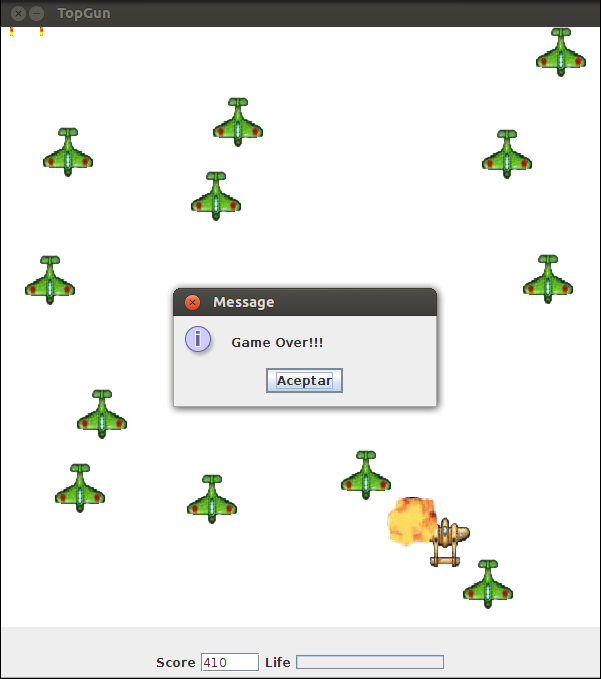
\includegraphics[scale= 0.72]{./cap4/caso_03.png}
}
\caption{Captura del juego Top Gun programado en JAVA}
\label{caso3}
\end{figure}

\subsection{Top Gun}
 
Continuando con los casos de estudio, el próximo es un programa JAVA llamado TopGun.java. Cuando este programa se ejecuta aparece un juego de aviones (ver figura \ref{caso3}), en este juego el usuario conduce un avión y es manejado desde el teclado. El objetivo consiste en en derribar la mayor cantidad de aviones enemigos y un contador suma puntos por cada avión derribado.
Este programa, posee un módulo de aproximadamente de 600 líneas que van a ser analizadas por la herramienta IDA.

Al igual que el caso de estudio anterior (Editor de texto), debido a que el programa TopGun.java contiene muchos ids, en la tabla \ref{tabla7} se lista el análisis de ids más relevantes de TopGun.\\

\noindent \textbf{Análisis de Resultados\\}

A diferencia de los casos de estudios antes vistos, en la tabla \ref{tabla7} se puede observar la presencia de ids capturados conformados por 3 palabras; algunos ejemplo de esto son: \textsf{LIFEprogressBar}, \textsf{hitShotEnemy}, \textsf{hitPlaneEnemy}.

En la división de ids persiste la tendencia en Greedy con respecto a Samurai, de separar mal algunos ids (ver caso de estudio anterior).

Las expansiones de ids en general están bastante precisas, cabe mencionar que los ids extraídos no presentan muchas dificultades en la traducción de las palabras completas que representan.

De los ids analizados (ver tabla \ref{tabla7} en las columnas Expansión desde Greedy y Expansión desde Samurai), las palabras que más frecuentemente aparecen están asociados al juego. De estos palabras se pueden nombrar, disparos, aviones, enemigos, imágenes, actualizar pantalla, movimiento. Estas palabras forman parte del Dominio del Problema en el que está enmarcado el programa TopGun.java.

%\begin{table}[ht!]
%\parbox{.40\linewidth}{
% 
%		\centering
%   		\begin{tabular}{| c | c |}  
%       \hline
%\textbf{Línea} & \textbf{Comentario} \\ \hline
%11&Attributes \\ \hline
%25&shoot number \\ \hline
%28&plane position \\ \hline
%32&plane movement \\ \hline
%35&Classes \\ \hline
%41&Constructor \\ \hline
%44&To close the window \\ \hline
%51&KeyListener for JFrame \\ \hline
%54&Status Panel \\ \hline
%62&Size \\ \hline
%66&initiate the enemies \\ \hline
%83&Focus in JFrame \\ \hline
%86&plane position \\ \hline
%88&x axe row \\ \hline
%89&y axe column \\ \hline
%96&start shooting \\ \hline
%98&plane's shot \\ \hline
%\end{tabular}
%}
%\hfill
%\parbox{.48\linewidth}{
% 
%		\centering
%   		\begin{tabular}{| c | c |}  
%       \hline
%\textbf{Línea} & \textbf{Comentario} \\ \hline
%247&clean \\ \hline
%249&set background color \\ \hline
%252&update the content \\ \hline
%%260&refresh the screen after delay 50 miliseconds \\ \hline
%271&drawing the plane \\ \hline
%298&check width height x y position \\ \hline
%307&plane's position \\ \hline
%310&enemy's position \\ \hline
%314&check the enemy and shot position \\ \hline
%330&if the shot is still active \\ \hline
%337&shot's position \\ \hline
%340&enemy's position \\ \hline
%344&check the enemy and shot position \\ \hline
%357&game classes. \\ \hline
%358&Launch the enemies \\ \hline
%385&shot's position \\ \hline
%393&TopGun class \\ \hline
%402&random position of enemy plane \\ \hline
%
%\end{tabular}
%}
%\caption{Comentarios extraídos por el AS ANTLR}\label{tabla9}
%\end{table}
%
%\begin{table}[h!]
%	
%		\centering
%   		\begin{tabular}{| c | c |}      
%       \hline
%  	   \textbf{Línea} & \textbf{Literal} \\ \hline
%  	   
%12&“Press Space button to Start” \\ \hline
%16&“Score” \\ \hline
%19&“Life” \\ \hline
%56&“Roman” \\ \hline
%72&“TopGun v 1.0” \\ \hline
%119&“0” \\ \hline
%125&“South” \\ \hline
%201&“Game Over!!!” \\ \hline
%203&“Message” \\ \hline
%234&“plane” \\ \hline
%235&“shot” \\ \hline
%236&“enemy” \\ \hline
%237&“exploit” \\ \hline  	   
%
%  \end{tabular} 
%	 
%   \caption{Literales extraídos por el AS ANTLR}
%   \label{tabla10}
%     
%\end{table} 


\begin{sidewaystable}[h!]
		\centering
   		\begin{tabular}{| c | c | c | c | c |}     
   		
       \hline
  	   \textbf{Id} & \textbf{Greedy} & \textbf{Samurai} & \textbf{Exp. desde Greedy} & \textbf{Exp. desde Samurai} \\ \hline
strt\_but&str--t--but&strt--but&start topgun but&start but\\ \hline
scoLabel&sco--label&sco--label&score label&score label\\ \hline
scotext&sco--text&sco--text&score text&score text\\ \hline
lifelabel&life--label&life--label&life label&life label\\ \hline
LIFEprogressBar&life--progress--bar&life--progress--bar&life progress background&life progress background\\ \hline
init&init&init&initiate&initiate\\ \hline
sn&sn&sn&shoot number&shoot number\\ \hline
pm&pm&pm&plane movement&plane movement\\ \hline
shot&shot&shot&shoot&shoot\\ \hline
lnEne&ln--en--e&ln--ene&launch enemies enemies&launch enemies\\ \hline
rfshScreen&rfs--h--screen&rfsh--screen&refresh hit screen&refresh screen\\ \hline
shoImage&sho--image&sho--image&shot images&shot images\\ \hline
eneImage&en--e--image&ene--image&enemies enemies images&enemies images\\ \hline
bangImage&bang--image&bang--image&bang images&bang images\\ \hline
tg&tg&tg&topgun&topgun\\ \hline
hitPlaneEnemy&hit--plane--enemy&hit--plane--enemy&height planes enemys&height planes enemys\\ \hline
intExp&int--exp&int--exp&int exploit&int exploit\\ \hline
enNum&en--nu--m&en--num&enemies number movement&enemies number\\ \hline
getYac&get--y--ac&get--yac&get yin active&get y axe column\\ \hline
getXar&get--xa--r&get--xar&get xa row&get x axe row\\ \hline
%Shot&shot&shot&Shoot&Shoot\\ \hline
ie&ie&ie&initiate enemies&initiate enemies\\ \hline
updatePlane&update--plane&update--plane&update planes&update planes\\ \hline
updateShot&update--shot&update--shot&update shoot&update shoot\\ \hline
hitShotEnemy&hit--shot--enemy&hit--shot--enemy&height shoot enemys&height shoot enemys\\ \hline
%ie&ie&ie&initiate enemies&initiate enemies\\ \hline
updatePlane&update--plane&update--plane&update planes&update planes\\ \hline
updateShot&update--shot&update--shot&update shoot&update shoot\\ \hline
keyReleased&key--released&key--released&keylistener released&keylistener released\\ \hline
   
   	\end{tabular}  
	 
   \caption{Parte del Análisis Realizado a los Ids de TopGun.java}
   \label{tabla7}
     
\end{sidewaystable} 

\clearpage %esto es necesario sino las tablas se van al final del capitulo